\documentclass[a4paper,titlepage]{article}

%PACKAGES
\usepackage[utf8]{inputenc}
\usepackage[T1]{fontenc}
\usepackage[english]{babel}
\usepackage{amsmath}
\usepackage{amssymb}
\usepackage{mathrsfs}
\usepackage{fancyhdr}
\usepackage{lmodern}
\usepackage{graphicx}
\usepackage{geometry}
\usepackage{fancybox}
\usepackage{textcomp}

%Symbole euro
\usepackage{eurosym}

%Listings : affichage code
\usepackage{listings}


%Elements de la page de garde
\begin{document}

\begin{titlepage}

\begin{figure}
\centering

\includegraphics[width=5cm]{logo-ulg.png}
\end{figure}



\title{
\vspace{0.2cm}
\LARGE{\textbf{Project 2 - Firewalls}} \\ \textsc{Introduction to Computer Security}
\author{\textbf{Floriane Magera} \small{(S111295})\\\textbf{Fabrice Servais} \small{(S111093})}\\
\date{March 27, 2015}
\rule{15cm}{1.5pt}
}

%\geometry{hmargin=2.5cm}
\end{titlepage}

%DOCUMENT
\pagestyle{fancy}
\lhead{Project 2 : Firewalls}
\rhead{Introduction to Computer Security}

%Page de garde
\maketitle


\section{Network topology}
\subsection{Explanation}
In order to draw the network, we supposed that the network was well structured : for example, a routing algorithm in the network would not have to use the longest prefix match method to find a route in the network, i.e each subnet is well defined by a range of IP addresses. We based our drawing only on the IP address. First we defined the different subnets, most of them were defined only by drawing the firewalls. Then we added all the devices in the right subnet. \\ \\

Then once the topology was defined, we tried to guess where should be the NAT's in the network. We know that the  PDNS server, SMTP server and the FTP server need to be accessible from the internet, and we also know that every user from the network must be unreachable from the internet. That is why we put one NAT in front of FW2 and one NAT before I2. We notice also that the SSH relay must be reachable from the internet, and for that reason we would configure a static mapping between its private and public address.


\subsection{Drawing}
\begin{center}
	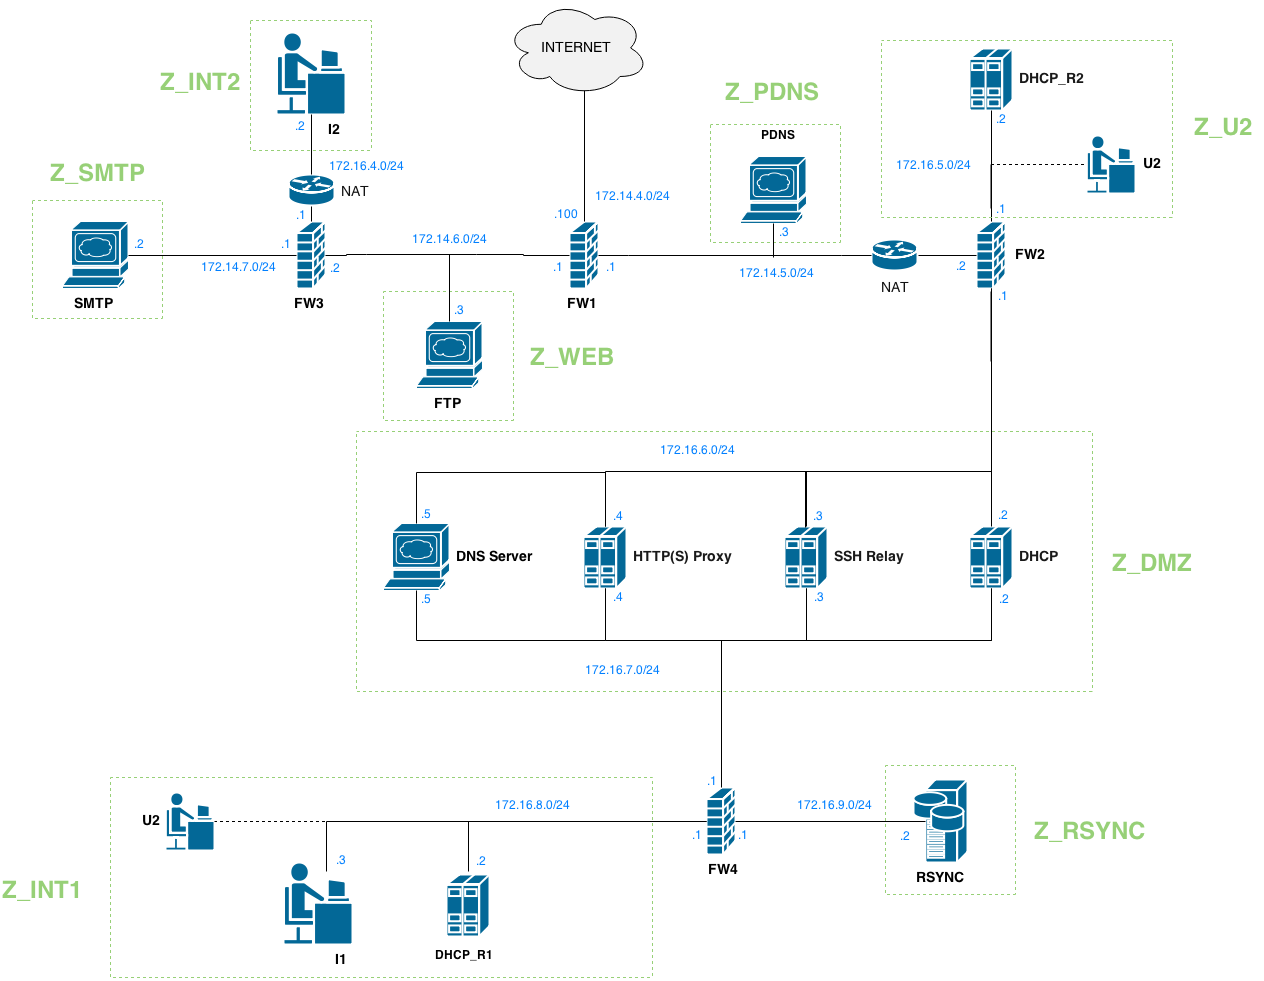
\includegraphics[scale=0.4]{ICS-Draw.png}
\end{center}
	


\end{document}
